%-----------------------------------------------------
% index key words
%-----------------------------------------------------
\index{line, parametric equation of line}
\index{area, area!triangle}

%-----------------------------------------------------
% name, leave blank
% title, if the exercise has a name i.e. Hilbert's matrix
% difficulty = n, where n is the number of stars
% origin = "\cite{ref}"
%-----------------------------------------------------
\begin{Exercise}[
name={},
title={}, 
difficulty=0,
origin={\cite{YL}}]
Given the line $(x,\;y,\;z)=(1+3t,\; 2+2t,\; 3+t)$ where $t\in\Re$ and point $P(3,\;2,\;1)$.
\Question Sketch the given line using $P_0$ the point on the line when $t=0$ and $P_1$ the point on the line when $t=1$, also sketch $P$.
\Question Using projections find area of the triangle defined by the points $P_0$, $P_1$ and $P$.
\Question Find the equation of the line which passes through the point $P$
and the closest point on the given line.
\end{Exercise}
\begin{Answer}
\Question\mbox{ }\\
% note the axes are reversed! 
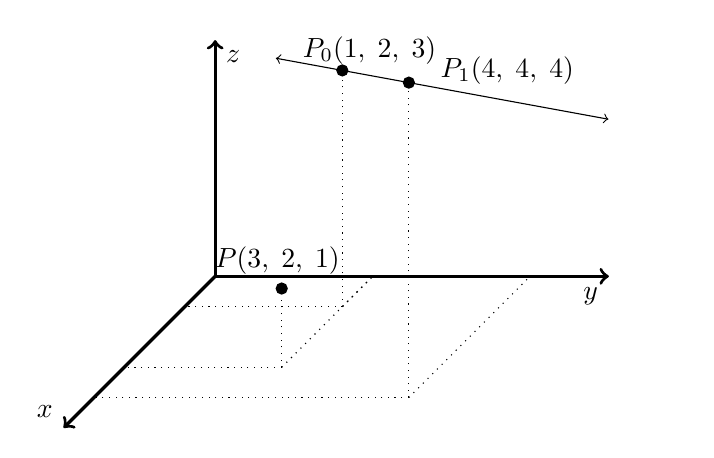
\begin{tikzpicture}%[tdplot_main_coords]
\draw[very thick,->] (0,0,0) -- (5,0,0) node[anchor=north east]{$y$};
\draw[very thick,->] (0,0,0) -- (0,3,0) node[anchor=north west]{$z$};
\draw[very thick,->] (0,0,0) -- (0,0,5) node[anchor=south east]{$x$};
\draw[<->] (0,2,-2) -- (10,7,13);
\draw[dotted] (2,0,1)--(0,0,1);
\draw[dotted] (2,0,1)--(2,0,0);
\draw[dotted] (2,0,1)--(2,3,1);

\draw[dotted] (4,0,4)--(0,0,4);
\draw[dotted] (4,0,4)--(4,0,0);
\draw[dotted] (4,0,4)--(4,4,4);

\node[text width = 3cm] at (3,3.25,1) {$P_0(1,\;2,\;3)$};
\filldraw (4,4,4) circle (2pt);
\node[text width = 3cm] at (6,4.25,4.25) {$P_1(4,\;4,\;4)$};
\filldraw (2,3,1) circle (2pt);

\draw[dotted] (2,0,3)--(0,0,3);
\draw[dotted] (2,0,3)--(2,0,0);
\draw[dotted] (2,0,3)--(2,1,3);
\node[text width = 3cm] at (2.75,1.45,3.25) {$P(3,\;2,\;1)$};
\filldraw (2,1,3) circle (2pt);
\end{tikzpicture}
\Question $2\sqrt{6}$
\Question $\vec{x}=(3,\;2,\;1) + t(2,\;-1,\;-4)$ where $t\in\Re$.
\end{Answer}
